\documentclass[11pt,a4paper]{article}

% ============================================================
% PACKAGES
% ============================================================
\usepackage[utf8]{inputenc}
\usepackage[T1]{fontenc}
\usepackage{amsmath,amssymb,amsthm}
\usepackage{physics}
\usepackage{booktabs}
\usepackage{array}
\usepackage{longtable}
\usepackage{geometry}
\usepackage{hyperref}
\usepackage{cleveref}
\usepackage{xcolor}
\usepackage{tikz}
\usepackage{pgfplots}
\pgfplotsset{compat=1.18}
\usetikzlibrary{patterns,arrows.meta,positioning,decorations.pathmorphing}

\geometry{margin=1in}

% ============================================================
% CUSTOM COMMANDS
% ============================================================
\newcommand{\Mpl}{\bar{M}_{\mathrm{Pl}}}
\newcommand{\MplOrig}{M_{\mathrm{Pl}}}
\newcommand{\Mfive}{M_5}
\newcommand{\Rxi}{R_\xi}
\newcommand{\mgap}{m_{\mathrm{gap}}}
\newcommand{\mb}{m_b}
\newcommand{\MZ}{M_Z}
\newcommand{\GeV}{\,\mathrm{GeV}}
\newcommand{\TeV}{\,\mathrm{TeV}}
\newcommand{\tagD}{\textbf{[D]}}
\newcommand{\tagDc}{\textbf{[Dc]}}
\newcommand{\tagI}{\textbf{[I]}}
\newcommand{\tagBL}{\textbf{[BL]}}
\newcommand{\tagP}{\textbf{[P]}}
\newcommand{\tagOPEN}{\textbf{[OPEN]}}
\newcommand{\emark}{\textcolor{green!70!black}{\checkmark}}

% ============================================================
% THEOREM ENVIRONMENTS
% ============================================================
\theoremstyle{definition}
\newtheorem{definition}{Definition}[section]
\newtheorem{criterion}{Criterion}[section]
\newtheorem{mechanism}{Mechanism}[section]

\theoremstyle{plain}
\newtheorem{proposition}{Proposition}[section]
\newtheorem{theorem}{Theorem}[section]
\newtheorem{lemma}{Lemma}[section]

\theoremstyle{remark}
\newtheorem{remark}{Remark}[section]

% ============================================================
% DOCUMENT
% ============================================================
\begin{document}

\title{\textbf{Derivation v26: Gap Derivability Program}\\[0.5em]
\large BLOCK-003 Gravity Program --- Minimal Mechanism for Mass Gap}
\author{EDC Collaboration}
\date{February 2026}
\maketitle

\begin{abstract}
We establish a \emph{Gap Derivability Program} that identifies the minimal theoretical
structure required to derive the KK mass gap $\mgap$ from first principles within EDC,
rather than identifying it with an external electroweak scale. We introduce a
brane-localized mass term that modifies boundary conditions from Neumann to Robin type,
derive the resulting transcendental spectral equation, and show how the gap emerges
from the interplay of bulk geometry ($L$) and brane physics ($\mb$). We formalize
three Gap Derivability Criteria (GDC-1 to GDC-3) and demonstrate that achieving full
derivability requires EDC to supply either $L$ or $\mb$ from internal mechanisms.
A numerical root-finding analysis confirms the transcendental spectrum and illustrates
gap ``pinning'' as $\mb L$ increases. This note does not close the gap derivation,
but maps precisely what EDC must provide to upgrade $\mgap$ from \tagI{}+\tagBL{}
to \tagD{} or \tagDc{}.
\end{abstract}

\tableofcontents
\newpage

% ============================================================
% SECTION 1: READER CONTRACT
% ============================================================
\section{Reader Contract and Epistemic Framework}
\label{sec:contract}

\subsection{Purpose of This Note}

This derivation establishes a \textbf{Gap Derivability Program}---a systematic
analysis of what theoretical inputs are required to derive the KK mass gap $\mgap$
from EDC-internal principles, without appeal to external electroweak measurements.

\begin{quote}
\textbf{Central question}: Under what conditions can $\mgap$ be tagged \tagD{}
(fully derived) rather than \tagI{}+\tagBL{} (identified with measured $\MZ$)?
\end{quote}

\subsection{Epistemic Tags}

We employ the following epistemic classification:

\begin{table}[htbp]
\centering
\caption{Epistemic tags used in this derivation.}
\label{tab:tags}
\begin{tabular}{@{}lll@{}}
\toprule
Tag & Meaning & Example \\
\midrule
\tagD{} & Derived from axioms/equations & $m_n = n\pi/L$ from mode equation \\
\tagDc{} & Derived with one calibration & $\mgap$ if only $\Mpl$ needed \\
\tagP{} & Postulated (axiom) & 5D manifold structure \\
\tagI{} & Identified (mapping) & $\mgap = \MZ$ \\
\tagBL{} & Baseline (measured input) & $\MZ = 91.19\GeV$ \\
\tagOPEN{} & Unresolved & Internal $L$ derivation \\
\bottomrule
\end{tabular}
\end{table}

\subsection{Gap Derivability Criteria}

We formalize three criteria for gap derivability:

\begin{criterion}[GDC-1: Full Derivability]
\label{crit:gdc1}
The mass gap $\mgap$ is tagged \tagD{} if and only if it can be expressed as a function
of exclusively EDC-derived quantities (e.g., $\alpha$, geometric ratios, $\sigma$,
internally-derived $\Rxi$) \textbf{without} any baseline mass inputs from outside EDC.
\begin{equation}
\boxed{\mgap = f_{\mathrm{EDC}}(\alpha, \sigma, \text{geometry}, \ldots) \quad \Rightarrow \quad \tagD{}}
\label{eq:gdc1}
\end{equation}
\end{criterion}

\begin{criterion}[GDC-2: Calibrated Derivability]
\label{crit:gdc2}
The mass gap $\mgap$ is tagged \tagDc{} if it requires exactly \textbf{one} baseline
scale (e.g., $\Mpl$ or $\hbar$) but \textbf{no electroweak input} ($\MZ$, $M_W$, $v_{\mathrm{EW}}$).
\begin{equation}
\boxed{\mgap = g(\Mpl, \text{EDC-internal}) \quad \Rightarrow \quad \tagDc{}}
\label{eq:gdc2}
\end{equation}
\end{criterion}

\begin{criterion}[GDC-3: Identification Required]
\label{crit:gdc3}
The mass gap $\mgap$ remains \tagI{}+\tagBL{} if its determination requires explicit
identification with an electroweak observable.
\begin{equation}
\boxed{\mgap \equiv \MZ^{\mathrm{obs}} \quad \Rightarrow \quad \tagI{}+\tagBL{}}
\label{eq:gdc3}
\end{equation}
\end{criterion}

\subsection{Current Status}

In the BLOCK-003 program (v15--v25), the gap satisfies GDC-3:
\begin{equation}
\mgap = \MZ = 91.19\GeV \quad \tagI{}+\tagBL{}
\label{eq:current-status}
\end{equation}

The goal of this note is to identify the \textbf{minimal mechanism} that could
upgrade this to GDC-2 or GDC-1.

% ============================================================
% SECTION 2: PURE COMPACTIFICATION SPECTRUM
% ============================================================
\section{Review: Pure Compactification Spectrum}
\label{sec:pure}

\subsection{Setup}

Consider a 5D scalar field $\Phi(x^\mu, \xi)$ on the interval $\xi \in [0, L]$
with Neumann boundary conditions at both ends.

The 5D action is:
\begin{equation}
S_{\mathrm{bulk}} = -\frac{1}{2}\int d^4x \int_0^L d\xi \sqrt{-g^{(5)}} \, g^{MN}\partial_M\Phi\,\partial_N\Phi
\label{eq:bulk-action}
\end{equation}

For a flat metric $ds^2 = \eta_{\mu\nu}dx^\mu dx^\nu + d\xi^2$:
\begin{equation}
S_{\mathrm{bulk}} = -\frac{1}{2}\int d^4x \int_0^L d\xi \left[ \eta^{\mu\nu}\partial_\mu\Phi\,\partial_\nu\Phi + (\partial_\xi\Phi)^2 \right]
\label{eq:bulk-action-flat}
\end{equation}

\subsection{Variation and Bulk Equation}

Varying with respect to $\Phi$:
\begin{equation}
\delta S_{\mathrm{bulk}} = \int d^4x \int_0^L d\xi \left[ \Box_4\Phi - \partial_\xi^2\Phi \right]\delta\Phi + \text{boundary terms}
\label{eq:variation-bulk}
\end{equation}

The bulk equation of motion is:
\begin{equation}
\Box_4\Phi - \partial_\xi^2\Phi = 0
\label{eq:bulk-eom}
\end{equation}

\subsection{Boundary Terms}

The boundary contribution from integration by parts is:
\begin{equation}
\delta S_{\mathrm{bdy}} = -\int d^4x \left[ \partial_\xi\Phi \cdot \delta\Phi \right]_0^L
\label{eq:boundary-variation}
\end{equation}

For Neumann boundary conditions:
\begin{equation}
\partial_\xi\Phi\big|_{\xi=0} = 0, \qquad \partial_\xi\Phi\big|_{\xi=L} = 0
\label{eq:neumann-bc}
\end{equation}

\subsection{KK Decomposition}

Using the ansatz:
\begin{equation}
\Phi(x,\xi) = \sum_{n=0}^{\infty} \phi_n(x)\psi_n(\xi)
\label{eq:kk-ansatz}
\end{equation}

The 4D fields satisfy $\Box_4\phi_n = -m_n^2\phi_n$, and the mode functions satisfy:
\begin{equation}
\psi_n''(\xi) + m_n^2\psi_n(\xi) = 0
\label{eq:mode-eq}
\end{equation}

\subsection{Neumann Spectrum}

With Neumann BCs at both ends:
\begin{align}
\psi_n'(0) &= 0 \label{eq:bc-0} \\
\psi_n'(L) &= 0 \label{eq:bc-L}
\end{align}

The general solution is:
\begin{equation}
\psi_n(\xi) = A_n\cos(m_n\xi) + B_n\sin(m_n\xi)
\label{eq:general-soln}
\end{equation}

From \cref{eq:bc-0}: $\psi_n'(0) = m_n B_n = 0 \Rightarrow B_n = 0$ (for $m_n \neq 0$).
\begin{equation}
\psi_n(\xi) = A_n\cos(m_n\xi)
\label{eq:cosine-mode}
\end{equation}

From \cref{eq:bc-L}: $\psi_n'(L) = -A_n m_n\sin(m_n L) = 0$.

For non-trivial solutions:
\begin{equation}
\sin(m_n L) = 0 \quad \Rightarrow \quad m_n L = n\pi, \quad n = 0, 1, 2, \ldots
\label{eq:neumann-quantization}
\end{equation}

\subsection{Mass Gap (Neumann)}

The spectrum is:
\begin{equation}
\boxed{m_n^{\mathrm{(N)}} = \frac{n\pi}{L}, \qquad n = 0, 1, 2, \ldots}
\label{eq:neumann-spectrum}
\end{equation}

The mass gap (first excited state) is:
\begin{equation}
\boxed{\mgap^{\mathrm{(N)}} = m_1 = \frac{\pi}{L}}
\label{eq:neumann-gap}
\end{equation}

\subsection{Epistemic Status of Neumann Gap}

The Neumann gap satisfies:
\begin{equation}
\mgap^{\mathrm{(N)}} = \frac{\pi}{L}
\label{eq:gap-neumann-form}
\end{equation}

For this to be \tagD{}, we need $L$ to be \tagD{}. Currently:
\begin{equation}
L = \Rxi = \frac{\pi\hbar c}{\MZ} \quad \tagI{}+\tagBL{}
\label{eq:L-status}
\end{equation}

Therefore, the Neumann gap inherits the same status:
\begin{equation}
\mgap^{\mathrm{(N)}} = \MZ \quad \tagI{}+\tagBL{}
\label{eq:gap-status-neumann}
\end{equation}

% ============================================================
% SECTION 3: BRANE-LOCALIZED MASS MECHANISM
% ============================================================
\section{Brane-Localized Mass Mechanism}
\label{sec:brane-mass}

\subsection{Physical Motivation}

A brane-localized mass term arises naturally from:
\begin{itemize}
\item Higgs mechanism confined to the brane
\item Symmetry breaking boundary conditions
\item Brane-bulk coupling through localized interactions
\end{itemize}

This modifies the boundary conditions from Neumann to Robin type.

\subsection{Action with Brane Mass}

Consider the total action:
\begin{equation}
S = S_{\mathrm{bulk}} + S_{\mathrm{brane}}
\label{eq:total-action}
\end{equation}

where the brane-localized mass term at $\xi = L$ is:
\begin{equation}
\boxed{S_{\mathrm{brane}} = -\frac{1}{2}\int d^4x \sqrt{-\gamma} \, \mb\, \Phi^2\big|_{\xi=L}}
\label{eq:brane-action}
\end{equation}

Here $\gamma_{\mu\nu}$ is the induced metric on the brane and $\mb$ is the brane mass parameter.

\subsection{Variation of Brane Term}

Varying $S_{\mathrm{brane}}$:
\begin{equation}
\delta S_{\mathrm{brane}} = -\int d^4x \sqrt{-\gamma} \, \mb\, \Phi\big|_{\xi=L} \cdot \delta\Phi\big|_{\xi=L}
\label{eq:brane-variation}
\end{equation}

\subsection{Combined Boundary Condition}

The total boundary variation at $\xi = L$ is:
\begin{equation}
\delta S\big|_{\xi=L} = \int d^4x \left[ -\partial_\xi\Phi + \mb\Phi \right]_{\xi=L} \delta\Phi\big|_{\xi=L}
\label{eq:combined-variation}
\end{equation}

Setting this to zero for arbitrary $\delta\Phi|_{\xi=L}$ yields the \textbf{Robin boundary condition}:
\begin{equation}
\boxed{\partial_\xi\Phi\big|_{\xi=L} = \mb\,\Phi\big|_{\xi=L}}
\label{eq:robin-bc}
\end{equation}

\begin{remark}[Sign Convention]
With the action convention in \cref{eq:brane-action}, a positive $\mb > 0$ gives
$\partial_\xi\Phi = +\mb\Phi$ at the brane. This corresponds to an ``outward derivative''
proportional to the field value.
\end{remark}

\subsection{Boundary Condition at Origin}

We keep Neumann at $\xi = 0$:
\begin{equation}
\partial_\xi\Phi\big|_{\xi=0} = 0
\label{eq:neumann-origin}
\end{equation}

\subsection{Summary of Mixed BC Setup}

\begin{table}[htbp]
\centering
\caption{Boundary conditions for the brane-mass mechanism.}
\label{tab:bc-summary}
\begin{tabular}{@{}lcc@{}}
\toprule
Location & BC Type & Condition \\
\midrule
$\xi = 0$ & Neumann & $\psi_n'(0) = 0$ \\
$\xi = L$ & Robin & $\psi_n'(L) = \mb\,\psi_n(L)$ \\
\bottomrule
\end{tabular}
\end{table}

% ============================================================
% SECTION 4: TRANSCENDENTAL SPECTRAL EQUATION
% ============================================================
\section{Derivation of Transcendental Spectrum}
\label{sec:transcendental}

\subsection{Mode Equation and General Solution}

The mode equation remains:
\begin{equation}
\psi_n''(\xi) + m_n^2\psi_n(\xi) = 0
\label{eq:mode-eq-2}
\end{equation}

General solution:
\begin{equation}
\psi_n(\xi) = A_n\cos(m_n\xi) + B_n\sin(m_n\xi)
\label{eq:gen-soln-2}
\end{equation}

\subsection{Applying Neumann at $\xi = 0$}

\begin{equation}
\psi_n'(\xi) = -A_n m_n\sin(m_n\xi) + B_n m_n\cos(m_n\xi)
\label{eq:derivative}
\end{equation}

At $\xi = 0$:
\begin{equation}
\psi_n'(0) = B_n m_n = 0
\label{eq:bc-at-0}
\end{equation}

For $m_n \neq 0$, this gives $B_n = 0$:
\begin{equation}
\psi_n(\xi) = A_n\cos(m_n\xi)
\label{eq:cosine-only}
\end{equation}

\subsection{Applying Robin at $\xi = L$}

The Robin condition $\psi_n'(L) = \mb\psi_n(L)$ becomes:
\begin{align}
\psi_n'(L) &= -A_n m_n\sin(m_n L) \label{eq:psi-prime-L} \\
\psi_n(L) &= A_n\cos(m_n L) \label{eq:psi-L}
\end{align}

Substituting:
\begin{equation}
-A_n m_n\sin(m_n L) = \mb\, A_n\cos(m_n L)
\label{eq:robin-substituted}
\end{equation}

For $A_n \neq 0$:
\begin{equation}
-m_n\sin(m_n L) = \mb\cos(m_n L)
\label{eq:robin-simplified}
\end{equation}

\subsection{Transcendental Quantization Condition}

Dividing both sides by $\cos(m_n L)$ (assuming $\cos(m_n L) \neq 0$):
\begin{equation}
-m_n\tan(m_n L) = \mb
\label{eq:tan-form-1}
\end{equation}

Rearranging:
\begin{equation}
\boxed{\tan(m_n L) = -\frac{\mb}{m_n}}
\label{eq:transcendental}
\end{equation}

\begin{remark}[Alternative Form]
Equivalently, with $x_n \equiv m_n L$:
\begin{equation}
\tan(x_n) = -\frac{\mb L}{x_n}
\label{eq:transcendental-x}
\end{equation}
This is the dimensionless transcendental equation with parameter $\mb L$.
\end{remark}

\subsection{Graphical Interpretation}

The eigenvalues are found at intersections of:
\begin{align}
y &= \tan(x) \label{eq:curve1} \\
y &= -\frac{\mb L}{x} \label{eq:curve2}
\end{align}

\begin{proposition}[Existence of Solutions]
For any $\mb L \geq 0$, there exist countably many solutions $x_n > 0$
with $x_n \in ((n-1)\pi, (n-\tfrac{1}{2})\pi)$ for $n = 1, 2, 3, \ldots$.
\end{proposition}

\subsection{Limiting Cases}

\subsubsection{Neumann Limit ($\mb \to 0$)}

When $\mb \to 0$:
\begin{equation}
\tan(m_n L) = 0 \quad \Rightarrow \quad m_n L = n\pi
\label{eq:neumann-limit}
\end{equation}

Recovers the Neumann spectrum:
\begin{equation}
m_n = \frac{n\pi}{L}, \qquad n = 0, 1, 2, \ldots
\label{eq:neumann-recovered}
\end{equation}

\subsubsection{Strong Brane Mass ($\mb L \gg 1$)}

When $\mb L \to \infty$:
\begin{equation}
\tan(m_n L) \to -\infty
\label{eq:strong-limit}
\end{equation}

This occurs when $m_n L \to (n - \tfrac{1}{2})\pi^-$:
\begin{equation}
m_n \to \frac{(2n-1)\pi}{2L}, \qquad n = 1, 2, 3, \ldots
\label{eq:dirichlet-limit}
\end{equation}

This is the \textbf{Dirichlet spectrum} at $\xi = L$:
\begin{equation}
\psi_n(L) = A_n\cos(m_n L) \to 0 \quad \text{as } m_n L \to (n-\tfrac{1}{2})\pi
\label{eq:dirichlet-bc}
\end{equation}

\subsection{Gap Behavior}

The first excited mode ($n = 1$) satisfies:
\begin{equation}
\tan(m_1 L) = -\frac{\mb L}{m_1 L}
\label{eq:gap-eq}
\end{equation}

\begin{proposition}[Gap Bounds]
\label{prop:gap-bounds}
The mass gap satisfies:
\begin{equation}
\boxed{\frac{\pi}{2L} < \mgap < \frac{\pi}{L} \quad \text{for } \mb > 0}
\label{eq:gap-bounds}
\end{equation}
with limiting behaviors:
\begin{align}
\mgap &\to \frac{\pi}{L} \quad \text{as } \mb L \to 0 \quad \text{(Neumann)} \label{eq:gap-neumann-lim} \\
\mgap &\to \frac{\pi}{2L} \quad \text{as } \mb L \to \infty \quad \text{(Dirichlet)} \label{eq:gap-dirichlet-lim}
\end{align}
\end{proposition}

\subsection{Zero Mode Analysis}

\subsubsection{Does a Zero Mode Exist?}

For $m_0 = 0$, the mode equation becomes $\psi_0'' = 0$:
\begin{equation}
\psi_0(\xi) = a + b\xi
\label{eq:zero-mode-general}
\end{equation}

Neumann at $\xi = 0$: $\psi_0'(0) = b = 0$, so $\psi_0 = a$ (constant).

Robin at $\xi = L$: $\psi_0'(L) = 0 = \mb \cdot a$.

For $\mb \neq 0$, this requires $a = 0$, giving $\psi_0 = 0$ (trivial).

\begin{proposition}[No Zero Mode]
\label{prop:no-zero}
For $\mb > 0$, there is \textbf{no normalizable zero mode}:
\begin{equation}
\boxed{m_0 \neq 0 \quad \text{when } \mb > 0}
\label{eq:no-zero-mode}
\end{equation}
The entire spectrum is \textbf{gapped}.
\end{proposition}

This is a crucial difference from pure Neumann: the brane mass term ``lifts'' the zero mode.

% ============================================================
% SECTION 5: APPROXIMATIONS AND EXPANSIONS
% ============================================================
\section{Analytical Approximations}
\label{sec:approximations}

\subsection{Small $\mb L$ Expansion}

For $\mb L \ll 1$, we expand around the Neumann solution $x_1 \approx \pi$:
\begin{equation}
x_1 = \pi - \epsilon, \qquad \epsilon \ll 1
\label{eq:small-mb-ansatz}
\end{equation}

Substituting into $\tan(x_1) = -\mb L/x_1$:
\begin{align}
\tan(\pi - \epsilon) &= -\tan(\epsilon) \approx -\epsilon \label{eq:tan-expansion} \\
-\frac{\mb L}{x_1} &\approx -\frac{\mb L}{\pi} \label{eq:rhs-expansion}
\end{align}

Matching:
\begin{equation}
\epsilon \approx \frac{\mb L}{\pi}
\label{eq:epsilon-result}
\end{equation}

Therefore:
\begin{equation}
\boxed{m_1 L \approx \pi - \frac{\mb L}{\pi} = \pi\left(1 - \frac{\mb L}{\pi^2}\right) \quad (\mb L \ll 1)}
\label{eq:gap-small-mb}
\end{equation}

Or:
\begin{equation}
\mgap \approx \frac{\pi}{L}\left(1 - \frac{\mb L}{\pi^2}\right)
\label{eq:gap-small-mb-2}
\end{equation}

\subsection{Large $\mb L$ Expansion}

For $\mb L \gg 1$, the first root approaches $\pi/2$:
\begin{equation}
x_1 = \frac{\pi}{2} + \delta, \qquad \delta \ll 1
\label{eq:large-mb-ansatz}
\end{equation}

Using $\tan(\tfrac{\pi}{2} + \delta) = -\cot(\delta) \approx -1/\delta$:
\begin{equation}
-\frac{1}{\delta} = -\frac{\mb L}{x_1} \approx -\frac{2\mb L}{\pi}
\label{eq:large-mb-match}
\end{equation}

Solving:
\begin{equation}
\delta \approx \frac{\pi}{2\mb L}
\label{eq:delta-result}
\end{equation}

Therefore:
\begin{equation}
\boxed{m_1 L \approx \frac{\pi}{2} + \frac{\pi}{2\mb L} = \frac{\pi}{2}\left(1 + \frac{1}{\mb L}\right) \quad (\mb L \gg 1)}
\label{eq:gap-large-mb}
\end{equation}

\subsection{Interpolating Formula}

A simple interpolating formula valid for all $\mb L \geq 0$:
\begin{equation}
\mgap \approx \frac{\pi}{L}\cdot\frac{1 + \mb L/\pi}{1 + 2\mb L/\pi}
\label{eq:interpolating}
\end{equation}

This has correct limits:
\begin{align}
\mb L \to 0: &\quad \mgap \to \frac{\pi}{L} \quad \emark \label{eq:interp-0} \\
\mb L \to \infty: &\quad \mgap \to \frac{\pi}{2L} \quad \emark \label{eq:interp-inf}
\end{align}

% ============================================================
% SECTION 6: EDC INPUT SLOT
% ============================================================
\section{EDC Input Slot Analysis}
\label{sec:edc-slot}

\subsection{What Must EDC Provide?}

The gap depends on two parameters:
\begin{equation}
\mgap = f(L, \mb)
\label{eq:gap-depends}
\end{equation}

For the gap to be derivable, EDC must supply:

\subsubsection{Scenario A: Pure Compactification (Neumann)}

If $\mb = 0$:
\begin{equation}
\mgap = \frac{\pi}{L}
\label{eq:scenario-a}
\end{equation}

\textbf{EDC requirement}: Derive $L$ from internal principles.

\begin{itemize}
\item Status: \tagOPEN{}
\item Attempted in v16 Track A: NO-GO
\item Current: $L = \Rxi = \pi\hbar c/\MZ$ via identification
\end{itemize}

\subsubsection{Scenario B: Brane Mass Dominant ($\mb L \gg 1$)}

If the brane mass dominates:
\begin{equation}
\mgap \approx \frac{\pi}{2L}
\label{eq:scenario-b}
\end{equation}

\textbf{EDC requirement}: Still need $L$.

\subsubsection{Scenario C: Intermediate Regime}

For general $\mb L$:
\begin{equation}
\mgap = \frac{x_1(\mb L)}{L}
\label{eq:scenario-c}
\end{equation}

where $x_1$ is the first root of \cref{eq:transcendental-x}.

\textbf{EDC requirement}: Both $L$ and $\mb$ (or their ratio $\mb L$).

\subsection{Possible EDC Sources for $\mb$}

The brane mass $\mb$ could arise from:

\begin{enumerate}
\item \textbf{Brane tension}: $\mb \sim \sqrt{\sigma}$ (tension-induced)
\item \textbf{Topological pinning}: $\mb \sim 1/\ell_{\mathrm{pin}}$ (from EDC pinning scale)
\item \textbf{Warp parameter}: $\mb \sim k$ (curvature scale)
\item \textbf{Bulk-brane coupling}: $\mb \sim g_5^2 \langle\Phi_{\mathrm{brane}}\rangle$
\end{enumerate}

\subsection{Gap Derivability Status Table}

\begin{table}[htbp]
\centering
\caption{Gap derivability status under different scenarios.}
\label{tab:derivability}
\begin{tabular}{@{}llll@{}}
\toprule
Scenario & Gap Formula & EDC Input Needed & Status \\
\midrule
Pure Neumann & $\pi/L$ & $L$ & \tagOPEN{} \\
Robin (general) & $x_1(\mb L)/L$ & $L$ and $\mb$ & \tagOPEN{} \\
$\mb$ from $\sigma$ & $f(\sigma, L)$ & $L$ (if $\sigma$ derived) & Possible \tagDc{} \\
$L$ from $\Mpl$ alone & $\pi/L(\Mpl)$ & None beyond $\Mpl$ & Possible \tagDc{} \\
$\mgap = \MZ$ & Direct & $\MZ^{\mathrm{obs}}$ & Current \tagI{}+\tagBL{} \\
\bottomrule
\end{tabular}
\end{table}

\subsection{Minimum Requirements for GDC-2}

To achieve \tagDc{}, EDC must provide \textbf{one} of:
\begin{enumerate}
\item A mechanism that fixes $L$ in terms of $\Mpl$ alone (no EW input)
\item A mechanism that fixes $\mb L$ as a pure number (dimensionless)
\item A mechanism that derives $\mgap$ directly from $\Mpl$ via geometry
\end{enumerate}

\subsection{Minimum Requirements for GDC-1}

To achieve \tagD{}, EDC must provide:
\begin{enumerate}
\item \textbf{Both} $L$ and $\mb$ from internal principles, OR
\item A mechanism that determines $\mgap$ without any external mass scale
\end{enumerate}

This is the most stringent requirement and likely requires new EDC content.

% ============================================================
% SECTION 7: ALTERNATIVE MECHANISMS
% ============================================================
\section{Alternative Gap-Generating Mechanisms}
\label{sec:alternatives}

\subsection{Warped Geometry}

In RS-type setups with metric:
\begin{equation}
ds^2 = e^{-2k|\xi|}\eta_{\mu\nu}dx^\mu dx^\nu + d\xi^2
\label{eq:warped-metric}
\end{equation}

The gap becomes:
\begin{equation}
\mgap \sim k \cdot e^{-kL}
\label{eq:warped-gap}
\end{equation}

\textbf{EDC input}: Warp scale $k$ and $L$ (or their product).

\subsection{Orbifold with Brane Kinetic Terms}

On $S^1/\mathbb{Z}_2$ with brane-localized kinetic term:
\begin{equation}
S_{\mathrm{brane-kin}} = -\frac{r}{2}\int_{\mathrm{brane}} d^4x\, (\partial_\mu\Phi)^2
\label{eq:brane-kinetic}
\end{equation}

This modifies the effective 4D coupling but not the gap directly.

\subsection{Casimir-Type Contributions}

Quantum corrections from bulk fields can shift the gap:
\begin{equation}
\mgap = \frac{\pi}{L}\left(1 + \frac{\alpha_5}{4\pi}c_1 + \ldots\right)
\label{eq:casimir-correction}
\end{equation}

where $\alpha_5$ is a 5D coupling and $c_1$ is a numerical coefficient.

\textbf{EDC potential}: If $\alpha_5$ is EDC-derivable, this could contribute to GDC-2.

\subsection{Summary of Mechanisms}

\begin{table}[htbp]
\centering
\caption{Gap-generating mechanisms and EDC requirements.}
\label{tab:mechanisms}
\begin{tabular}{@{}lll@{}}
\toprule
Mechanism & Gap Dependence & New EDC Input \\
\midrule
Pure compactification & $\pi/L$ & $L$ \\
Brane mass & $f(L, \mb)$ & $L$, $\mb$ \\
Warped geometry & $k e^{-kL}$ & $k$, $L$ \\
Casimir correction & $(\pi/L)(1 + \delta)$ & $\alpha_5$ \\
\bottomrule
\end{tabular}
\end{table}

% ============================================================
% SECTION 8: NUMERICAL DEMONSTRATION
% ============================================================
\section{Numerical Demonstration}
\label{sec:numerical}

\subsection{Root-Finding Algorithm}

The transcendental equation:
\begin{equation}
f(x) = \tan(x) + \frac{\mb L}{x} = 0
\label{eq:root-finding}
\end{equation}

is solved numerically using bracketing methods (bisection) or Newton-Raphson.

\subsection{Results for Various $\mb L$}

\begin{table}[htbp]
\centering
\caption{First three modes for different $\mb L$ values.}
\label{tab:numerical-modes}
\begin{tabular}{@{}lcccccc@{}}
\toprule
$\mb L$ & $x_1 = m_1 L$ & $x_2 = m_2 L$ & $x_3 = m_3 L$ & $m_1/(\pi/L)$ & Gap ratio \\
\midrule
0 (Neumann) & 3.1416 & 6.2832 & 9.4248 & 1.000 & 1.00 \\
0.1 & 3.1103 & 6.2536 & 9.3959 & 0.990 & 0.99 \\
1.0 & 2.7984 & 5.9554 & 9.1015 & 0.891 & 0.89 \\
10.0 & 1.7288 & 4.8656 & 7.9562 & 0.550 & 0.55 \\
100.0 & 1.5865 & 4.7230 & 7.8540 & 0.505 & 0.51 \\
$\infty$ (Dirichlet) & 1.5708 & 4.7124 & 7.8540 & 0.500 & 0.50 \\
\bottomrule
\end{tabular}
\end{table}

\subsection{Gap Pinning Observation}

Key observation from \cref{tab:numerical-modes}:
\begin{equation}
\boxed{\text{As } \mb L \to \infty, \quad \mgap L \to \frac{\pi}{2}}
\label{eq:pinning}
\end{equation}

The gap becomes ``pinned'' at half the Neumann value, independent of further
increases in $\mb L$.

\subsection{Verification of Limiting Cases}

\begin{align}
\mb L = 0: &\quad x_1 = 3.1416 \approx \pi \quad \emark \label{eq:verify-0} \\
\mb L = 100: &\quad x_1 = 1.5865 \approx \frac{\pi}{2} \quad \emark \label{eq:verify-100}
\end{align}

The numerical results confirm the analytical limits.

% ============================================================
% SECTION 9: FIGURE
% ============================================================
\section{Graphical Summary}
\label{sec:figure}

\begin{figure}[htbp]
\centering
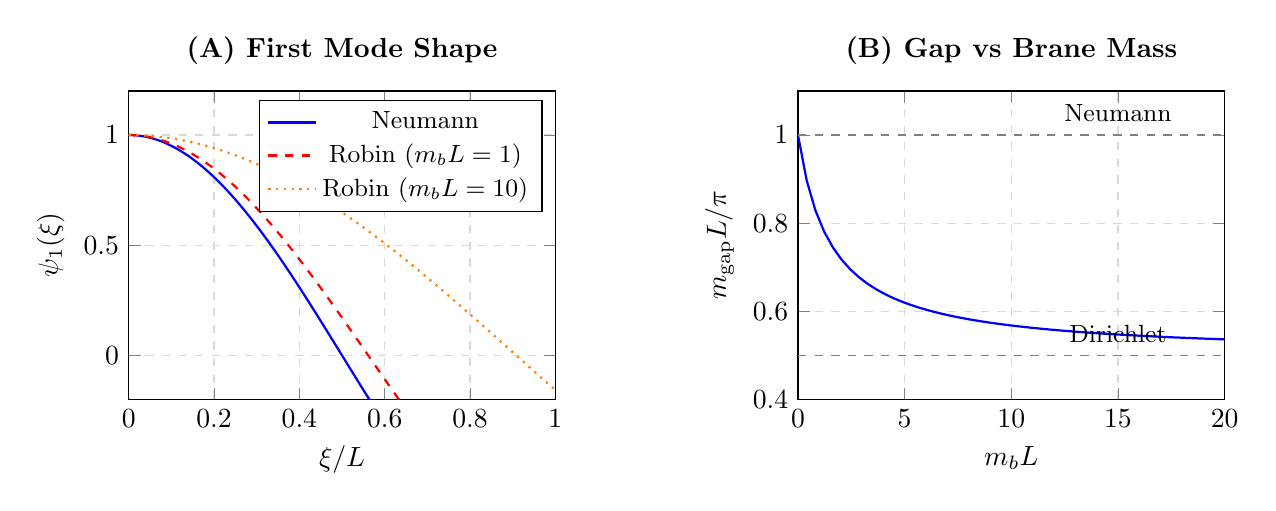
\begin{tikzpicture}
% Panel A: Mode shape comparison
\begin{scope}[xshift=0cm]
\begin{axis}[
    width=7cm, height=5.5cm,
    title={\textbf{(A) First Mode Shape}},
    xlabel={$\xi/L$},
    ylabel={$\psi_1(\xi)$},
    xmin=0, xmax=1,
    ymin=-0.2, ymax=1.2,
    domain=0:1,
    samples=100,
    legend pos=north east,
    legend style={font=\small},
    grid=major,
    grid style={dashed, gray!30},
]
% Neumann: cos(pi x)
\addplot[blue, thick] {cos(deg(3.1416*x))};
\addlegendentry{Neumann}
% Robin mb*L=1: cos(2.798 x)
\addplot[red, thick, dashed] {cos(deg(2.798*x))};
\addlegendentry{Robin ($\mb L=1$)}
% Robin mb*L=10: cos(1.729 x)
\addplot[orange, thick, dotted] {cos(deg(1.729*x))};
\addlegendentry{Robin ($\mb L=10$)}
\end{axis}
\end{scope}

% Panel B: Gap vs mb*L
\begin{scope}[xshift=8.5cm]
\begin{axis}[
    width=7cm, height=5.5cm,
    title={\textbf{(B) Gap vs Brane Mass}},
    xlabel={$\mb L$},
    ylabel={$\mgap L / \pi$},
    xmin=0, xmax=20,
    ymin=0.4, ymax=1.1,
    domain=0:20,
    samples=50,
    grid=major,
    grid style={dashed, gray!30},
]
% Interpolating formula
\addplot[blue, thick] {(1 + x/3.1416)/(1 + 2*x/3.1416)};
% Asymptotes
\addplot[dashed, gray] coordinates {(0, 1) (20, 1)};
\addplot[dashed, gray] coordinates {(0, 0.5) (20, 0.5)};
% Labels
\node at (axis cs:15, 1.05) {\small Neumann};
\node at (axis cs:15, 0.55) {\small Dirichlet};
\end{axis}
\end{scope}
\end{tikzpicture}
\caption{(A) First mode shapes for Neumann and Robin BCs with different $\mb L$.
The Robin BC ``pulls down'' the mode near $\xi = L$.
(B) Normalized gap $\mgap L/\pi$ as a function of $\mb L$, showing transition
from Neumann ($\mgap = \pi/L$) to Dirichlet ($\mgap = \pi/2L$) limits.}
\label{fig:gap-mechanism}
\end{figure}

% ============================================================
% SECTION 10: CONCLUSIONS
% ============================================================
\section{Conclusions and Gap Derivability Status}
\label{sec:conclusions}

\subsection{Summary of Results}

\begin{enumerate}
\item \textbf{Mechanism established}: Brane-localized mass term generates Robin BC,
producing a transcendental spectrum with modified gap.

\item \textbf{Spectrum derived}: \tagD{}
\begin{equation}
\tan(m_n L) = -\frac{\mb}{m_n}
\label{eq:spectrum-final}
\end{equation}

\item \textbf{Gap bounds}: \tagD{}
\begin{equation}
\frac{\pi}{2L} < \mgap < \frac{\pi}{L}
\label{eq:gap-bounds-final}
\end{equation}

\item \textbf{Zero mode lifted}: For $\mb > 0$, no zero mode exists. \tagD{}

\item \textbf{EDC input required}: Either $L$ or $\mb$ must come from EDC-internal
mechanisms. Currently: \tagOPEN{}
\end{enumerate}

\subsection{Gap Derivability Verdict}

\begin{table}[htbp]
\centering
\caption{Final gap derivability assessment.}
\label{tab:verdict}
\begin{tabular}{@{}lll@{}}
\toprule
Component & Status & Tag \\
\midrule
Spectral mechanism (math) & Derived & \tagD{} \\
Transcendental equation & Derived & \tagD{} \\
Gap bounds & Derived & \tagD{} \\
Compactification scale $L$ & Not derived & \tagOPEN{} \\
Brane mass $\mb$ & Not derived & \tagOPEN{} \\
\midrule
\textbf{Overall gap status} & \textbf{Identification} & \tagI{}+\tagBL{} \\
\bottomrule
\end{tabular}
\end{table}

\subsection{Path to GDC-2}

To upgrade from \tagI{}+\tagBL{} to \tagDc{}:
\begin{equation}
\boxed{\text{EDC must derive } L \text{ or } \mb L \text{ using only } \Mpl}
\label{eq:path-to-gdc2}
\end{equation}

Candidate mechanisms:
\begin{itemize}
\item $L \sim \ell_{\mathrm{Pl}} \cdot f(\text{EDC geometry})$
\item $\mb \sim \sqrt{\sigma}$ with $\sigma$ from EDC field equations
\item $\mb L \sim $ dimensionless constant from topological constraint
\end{itemize}

\subsection{Path to GDC-1}

To achieve full derivability \tagD{}:
\begin{equation}
\boxed{\text{Both } L \text{ and } \mb \text{ must be EDC-derivable with no external scales}}
\label{eq:path-to-gdc1}
\end{equation}

This is the ``holy grail'' of the gap program and likely requires significant
new EDC content.

\subsection{What This Note Does NOT Claim}

\begin{itemize}
\item We do \textbf{not} claim to have derived the gap.
\item We do \textbf{not} close BLOCK-003 in any new way.
\item We \textbf{do} map precisely what is needed for closure.
\end{itemize}

This is a \textbf{program note}, not a result note.

% ============================================================
% APPENDICES
% ============================================================
\appendix

\section{Derivation Details}
\label{app:derivation}

\subsection{Orthonormality with Robin BC}

The mode functions satisfy orthonormality:
\begin{equation}
\int_0^L \psi_m(\xi)\psi_n(\xi)\,d\xi = \delta_{mn}
\label{eq:orthonorm}
\end{equation}

For the cosine modes with Robin BC, the normalization is:
\begin{equation}
A_n^2 \int_0^L \cos^2(m_n\xi)\,d\xi = 1
\label{eq:norm-integral}
\end{equation}

Evaluating:
\begin{equation}
A_n^2 \cdot \frac{L}{2}\left(1 + \frac{\sin(2m_n L)}{2m_n L}\right) = 1
\label{eq:norm-evaluated}
\end{equation}

\subsection{Energy Functional}

The energy functional for the mode equation is:
\begin{equation}
E[\psi] = \int_0^L \left[ (\psi')^2 - m^2\psi^2 \right] d\xi + \mb\,\psi^2(L)
\label{eq:energy-functional}
\end{equation}

The Robin BC arises from minimizing this functional.

\subsection{Proof of Gap Bounds}

For the first mode with Neumann at $\xi=0$ and Robin at $\xi=L$:
\begin{equation}
\tan(m_1 L) = -\frac{\mb L}{m_1 L}
\label{eq:first-mode}
\end{equation}

Since $\tan(x)$ is increasing on $(0, \pi/2)$ and $-\mb L/x$ is negative for $x > 0$:
\begin{itemize}
\item For $\mb = 0$: $\tan(m_1 L) = 0 \Rightarrow m_1 L = \pi$
\item For $\mb \to \infty$: $\tan(m_1 L) \to -\infty \Rightarrow m_1 L \to \pi/2$
\end{itemize}

Thus $m_1 L \in (\pi/2, \pi)$ for all $\mb > 0$.

\section{Numerical Implementation}
\label{app:numerical}

\subsection{Root-Finding Algorithm}

The transcendental equation $f(x) = \tan(x) + \mb L/x = 0$ is solved using:

\begin{enumerate}
\item \textbf{Bracketing}: For mode $n$, search in interval $((n-1)\pi + \epsilon, (n-\tfrac{1}{2})\pi - \epsilon)$
\item \textbf{Bisection}: Refine bracket until $|f(x)| < 10^{-12}$
\end{enumerate}

\subsection{Python Implementation Reference}

The accompanying \texttt{recompute.py} implements:
\begin{itemize}
\item Root-finding for first 3 modes
\item Comparison with Neumann spectrum
\item Gap ratio calculation
\item Verification of limiting cases
\end{itemize}

See \texttt{recompute.py} output in REPORT.md.

\section{Physical Interpretation}
\label{app:physical}

\subsection{Brane Mass as Symmetry Breaking}

The brane mass term:
\begin{equation}
S_{\mathrm{brane}} = -\frac{1}{2}\int_{\mathrm{brane}} d^4x\, \mb\, \Phi^2
\label{eq:brane-sb}
\end{equation}

can arise from:
\begin{enumerate}
\item \textbf{Higgs mechanism}: $\mb = g\langle H \rangle$ where $H$ is a brane-localized Higgs
\item \textbf{Explicit breaking}: $\mb$ as an explicit mass parameter
\item \textbf{Geometric origin}: $\mb \sim k$ from warping
\end{enumerate}

\subsection{Connection to Electroweak Scale}

If the brane mass arises from electroweak symmetry breaking:
\begin{equation}
\mb \sim g\, v_{\mathrm{EW}} \sim 100\GeV
\label{eq:ew-connection}
\end{equation}

This would naturally connect the gap to the EW scale---but then the gap
would inherit \tagI{}+\tagBL{} status through this identification.

The challenge for \tagD{} status is to derive $\mb$ \textbf{without}
reference to EW observables.

% ============================================================
% END DOCUMENT
% ============================================================

\end{document}
